%cSpell:ignore Erol,Sezgin,fancyhdr, hheadheighti,hheadsepi,hfootheighti,graphicx, hfootskipi, Gavrilita, Mihail, AMOO, totalheight, keepaspectratio,UML's, kata, codewars, OOAD, COFFE,ERLANG,caml, kotlin,haskel, ruby, superclass, 
\documentclass[12pt]{article}
%\usepackage[english]{babel}
%actually it works without this package//// cuz it is in english by default... it might be useful //// but not here
% \usepackage{natbib}
% \usepackage{biblatex}

% \usepackage[backend=biber]{biblatex}

%\usepackage{url}
%idk what for it is here, it is not what it seems to be, fuck it
%%\usepackage[document]{ragged2e} 
%%to justify
% i dont use it anymore
\usepackage[utf8]{inputenc}
%%%\usepackage{amsmath}
%%useless for this report... it's for math stuff
\usepackage{graphicx}
%This package enables the user to the importation of graphics into a .tex file and, apart from the usual sizing and rotational facilities, also enables the user to crop or trim an image as desired (e.g., to get rid of surrounding blank margins). The graphicx package is useful if you need to use only a part of a complete image. 
\graphicspath{{images/}}
%% includes pics inside image folder
\usepackage{parskip}
%%this shit . In the document body, don't use \parskip but a blank line to separate paragraphs.there's normally no need to add manual line breaks (\\) in the text.

\usepackage{vmargin}
%%LaTeX package which introduces paper sizes and provides macros for setting document margins. 
\usepackage{enumerate} 
%enumeration of elements  
\usepackage{caption}
%%this is for figures
\usepackage{float}
%% to position exactly the figure 
\usepackage{fancyhdr}
%%To customize the footer and header in your document first import the package fancyhdr with 
% \addbibresource{lab4.bib}
% \bibliography{my_bibliography.bib} 
\PassOptionsToPackage{hyphens}{url}\usepackage{hyperref}
\hypersetup{
    colorlinks=true,
    linkcolor=blue,
    filecolor=magenta,      
    urlcolor=cyan,
}

\renewcommand{\theenumii}{\arabic{enumii}}
\setmarginsrb{3 cm}{2.5 cm}{3 cm}{2.5 cm}{1 cm}{1.5 cm}{1 cm}{1.5 cm}
%%\setmarginsrb{hleftmargini}{htopmargini}{hrightmargini}{hbottommargini}% {hheadheighti}{hheadsepi}{hfootheighti}{hfootskipi
\title{PPE Laboratory 2}								
\author{Sezgin E}							
\makeatletter
%%The \makeatletter command temporarily defines »@« as a normal character to enable changes to internal LaTeX macros outside packages (STY) or classes (CLS).
\let\thetitle\@title
%%\let allows you to copy the content of a command into a new command.
\let\theauthor\@author
%%Thus \let\foo\bar defines \foo to have the value that \bar had at the point of definition.
\makeatother
% With \makeatother this process is reversed and the »@« is set to its original character category (other). The »@« is used to protect the internal LaTeX macros. Hence you should be very careful when using these two commands.
\pagestyle{fancy}
%%After that, the "fancy" style is set by \pagestyle{fancy}
\fancyhf{}
%%The command \fancyhf{} clears the header and footer, otherwise the elements of the default "plain" page style will appear. 
\rhead{\theauthor}
%%Prints the text included inside the braces on the right side of the header. 
\lhead{\thetitle}
%%Prints the text set inside the braces on the left side of the header.
\cfoot{\thepage}
%%\cfoot{Page \thepage}  Prints the word "Page" and next the page number which is automatically set by \thepage on the center of the footer. 
        
\begin{document}
        
        %%%%%%%%%%%%%%%%%%%%%%%%%%%%%%%%%%%%%%%%%%%%%%%%%%%%%%%%%%%%%%%%%%%%
        
        \begin{titlepage}
                \centering
                \vspace*{0.5 cm}
                
\includegraphics[scale = 0.11]{LOGO_UTM.jpg}\\[1.0 cm]	% University Logo
                %% Importing a graphic is done by using the command \includegraphics[key1=...,key2=...,etc.]{filename} Optional parameters—called “keys”—enable the figure to be resized, rotated, cropped, trimmed, etc. These keys and their functions are listed below. 
                %• scale = number — a magnification factor 
                %• width = length — the width to which the figure should be scaled1
                %• height = length — the height to which the figure should be scaled2 
                %• totalheight = length — height plus depth of figure (to be used if figure is rotated) 
                %• keepaspectratio = true/false — maintains the height/width ratio 
                %• angle = number — angle (in degrees) by which the figure is to be rotated counterclockwise 
                %• origin = location3 — the point about which rotation is to occur %• draft = true/false — prevents figure from being imported, but created a named box with the dimensions of the figure (this option is used to speed up processing) 
                %• clip = true/false — excludes whatever is outside the bounding box 
                \textsc{\LARGE Technical University of Moldova}\\[2.0 cm]%%\textsc{example text} will display the example text as small caps. All of the letters will be capitalized/uppercase, but they are going to be similar in size to a lowercase letter.	
                % University Name
                \textsc{\Large 20.05.2018}\\[0.5 cm]		% Course Code

                \rule{\linewidth}{0.2 mm} \\[0.4 cm]
                %%The \rule command in normal use produces a simple black box: \rule[raise]{width}{thickness} This is useful for drawing vertical and horizontal lines.

                { \huge \bfseries \thetitle}\\
                %%Anyway, the \bfseries bold the rest of my document, even though I'm using curly braces.
                \rule{\linewidth}{0.2 mm} \\[1.5 cm]
                
                \begin{minipage}{0.4\textwidth}
                        \begin{flushleft} \large
                                \emph{Submitted To:}\\
                                Coslets Mihail\\
                %%If you want to emphasize a word or some text, use \emph. Don't just make the text italic or bold. If needed, you may change the behavior of \emph whenever you wish in the preamble and the whole document will be adjusted accordingly.
                Asst. Univ.\\
                Computer Science Department\\
                            \end{flushleft}
                            \end{minipage}~
                            \begin{minipage}{0.4\textwidth}
                
                            \begin{flushright} \large
                            \emph{Submitted By :} \\
                            Sezgin Erol\\
                
                Group FAF-161\\
                Semester 2\\
                    \end{flushright}
                
                \end{minipage}\\[2 cm]
                
                \vfill Chisinau 2018\\  
        \end{titlepage}
        
        %%%%%%%%%%%%%%%%%%%%%%%%%%%%%%%%%%%%%%%%%%%%%%%%%%%%%%%%%%%%%%%%%%%%
        \pagebreak
        %\tableofcontents
        \subsection*{Title:}
        \subsubsection*{Advanced Form Elements. Child Windows. Basics of Working With Keyboard.. }
        \subsection*{Contents:}
        \begin{itemize}
                \item The Keyboard;
                \item Child Window Controls;
                \item Menus and Other Resources;
                \begin{itemize}
                        \item Scroll Bar;
                        \item Listbox;
                \end{itemize}
                \item Dialog Boxes.
        \end{itemize}
       
        \subsection*{Mandatory Objectives:}
        \begin{itemize}
                \item Display a dialog box on some event (ex. on clicking some button);
                \item Add a system menu to your application with at least 3 items (add actions to that items);
                \item Add a scroll bar that will change any visible parameter of any other element (color of a text);
                \item Hook keyboard input. Add 2 custom events for 2 different keyboard combinations (ex. change window background on ctrl+space).
        \end{itemize}

        \subsection*{Objectives With points:}
        \begin{itemize}
                \item Add a listbox and attach some events when any element is accessed (clicked) ;
                \item Add 2 scroll bars that will manage main window size or position;
                \item Customize your application by adding an icon and using different cursor in application ;
                \item Use a scroll bar to scroll through application working space. Scroll should appear only when necessary (eg. when window width is smaller than 300px) .
        \end{itemize}


        \subsection*{Tasks:}
        During This Laboratory Work i Created System Menu With Elements like "File", "Visual Settings" and "Info" and I added Actions. So If user press Random background Color in visual settings the default color of desktop Application will be changed to random one. Pressing "Info" Will appear Window with Information Who is the Author of these lab.
        \begin{figure}[H]
                \centering
                
\includegraphics[width=.5\textwidth]{img1.png}
                \caption{The menu}
        \end{figure}
        \vspace{0.5 cm}

        Is present the listbox where i manually added few messages, during application running user can add new or delete existent ones
        \begin{figure}[H]
                \centering
                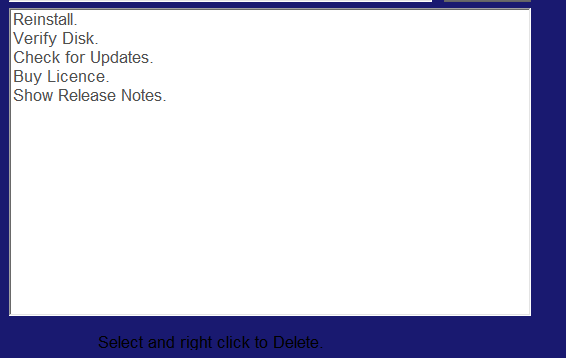
\includegraphics[width=.5\textwidth]{img3.png}
                \caption{ListBox}
        \end{figure}
        \vspace{0.5 cm}
         
       
        
        I Added the scroll bar, using it user will change the visibility of The text in upper Box;
        \begin{figure}[H]
                \centering
                
\includegraphics[width=.5\textwidth]{img2.png}
                \caption{The Scroll bar}
        \end{figure}
        \vspace{0.5 cm}
        Also there is Dialog Box showing the current Date, it appears after pressing "The Date" button
        \begin{figure}[H]
                \centering
                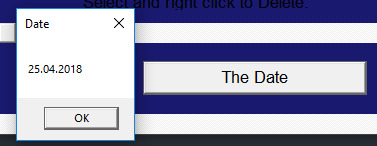
\includegraphics[width=.5\textwidth]{img4.png}
                \caption{DialogBox}
        \end{figure}
        \vspace{0.5 cm}
        Also i Addd 2 scroll Bars, on left ang right sides which manage the Window size, also added Custom Cursor and Icon for application. I implemented 2 Hot Keys "Alt + L" for menu item "Info" and "Alt + " for "Shut Down"
        \begin{figure}[H]
                \centering
                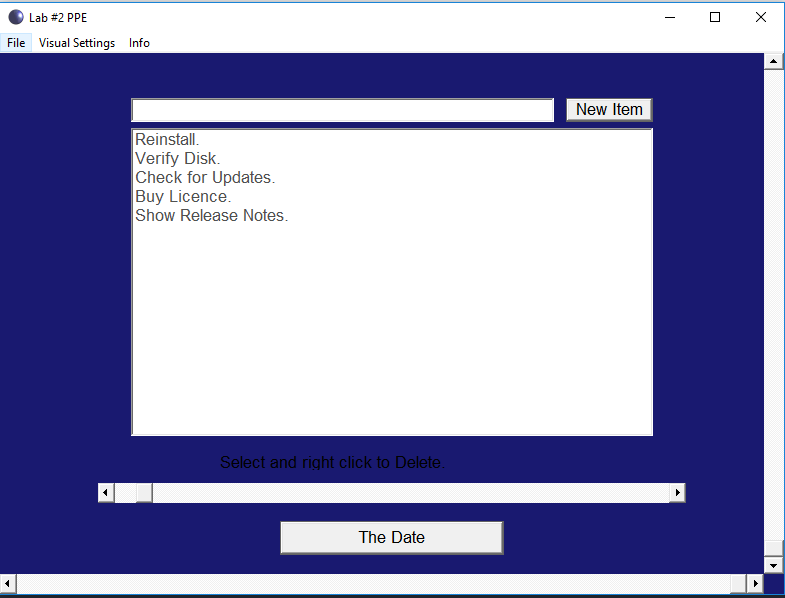
\includegraphics[width=.5\textwidth]{img5.png}
                \caption{The overall Image}
        \end{figure}
        \vspace{0.5 cm}
        \newpage
        \subsection*{Conclusion}
        During This lab work i Understand the key features of WinApi Like list boxes, Menu, and how to add custom elements. The hardest part was repositioning all window elements on scrolling.
        

 
\medskip
 
\begin{thebibliography}{9}

        \bibitem{sec1}
        Section I, Chapter 6

        \bibitem{sec2}
        Section I, Chapter 9

        \bibitem{sec3}
        Section I, Chapter 10

        \bibitem{sec4}
        Section I, Chapter 11
      

\end{thebibliography}
                
\end{document}